\section{Iterators}

Browsing on Containers

\subsection{Iterators}

\subsubsection{What is an Iterator?}

Iterators are special object that understand the \textbf{iterator protocol}:

\begin{itemize}
	\item \_\_iter\_\_ to build the iterator structure
	\item \_\_next\_\_ to get the next elemetn in the container, and
	\item StopIteratorion exeption to notify when datain container are finished
\end{itemize}

Generators are a special case of iterators:

\begin{lstlisting}[language=Python]
class Fib:
	'''iterator that yields numbers in the Fibonacci sequence'''
	def __init__(self, max):
		self.max = max
	def __iter__(self):
		self.a = 0
		self.b = 1
		return self
	def __next__(self):
		fib = self.a
		if fib > self.max: raise StopIteration
		self.a, self.b = self.b, self.a + self.b
		return fib
		
if __name__ == "__main__":
	f = Fib(1000)
	for i in f: print(i)
\end{lstlisting}

\subsubsection{Lazy Pluralize}

\begin{lstlisting}[language=Python]
class LazyRules:
	def __init__(self, rules_filename):
		self.pattern_file = open(rules_filename, encoding='utf-8')
		self.cache = []
	def __iter__(self):
		self.cache_index = 0
		return self
	def __next__(self):
		self.cache_index += 1
		if len(self.cache) >= self.cache_index:
			return self.cache[self.cache_index - 1]
		if self.pattern_file.closed: raise StopIteration
		line = self.pattern_file.readline()
		if not line:
			self.pattern_file.close()
			raise StopIteration
		pattern, search, replace = line.split(None, 3)
		funcs = build_match_and_apply_functions(pattern, search, replace)
		self.cache.append(funcs)
		return funcs
rules = LazyRules()
\end{lstlisting}

\begin{itemize}
	\item minimal startup cost: just instantiating a class and open a file
	\item maximum performance: the file is read on demand and never re-read
	\item code and data separation: patterns are stored on a file separated from the code 
\end{itemize}

\subsubsection{Cryptatithms}
The riddle:

\begin{center}
HAWAII + IDAHO + IOWA + OHIO == STATES
\end{center}

is a \textbf{cryptarithms}

\begin{itemize}
	\item the letters spell out actual words and a meaningful sentence
	\item each letter can be translated to a digit (0-9) no initial can be translated to 0
	\item to the same letter corresponds the same digit along the whole
sentence and no digit can be associated to two different letters
	\item the resulting arithmetic equation represents a valid and correct equation
\end{itemize}

\begin{center}
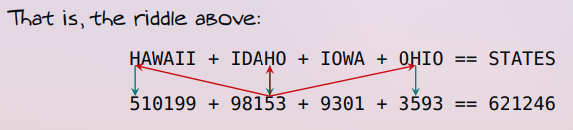
\includegraphics[scale=0.3]{4-iterators-cryptarithms}
\end{center}

\subsubsection{Cryptatithms: the solution}

How canwe face the riddle automatic solution?

A \textbf{brute force} approach.

First step consists of organizin the data
\begin{itemize}
	\item to find t he words that need to be translated
	\item to determine which characters compose such a sentence 
	\item to determine which characters are at the beginning of the words
\end{itemize}

Then, we look for the solution, if any, by
\begin{itemize}
	\item generating every possible permutation of ten digits (0-9)
	\item skimming those permutations with 0 associated to an initial
	\item  trying if the remaining permutations represent a valid solution
\end{itemize}

\begin{lstlisting}[language=Python]
import re, itertools, sys
def solve(puzzle):
	words = re.findall('[A-Z]+', puzzle.upper())
	unique_characters = set(''.join(words))
	assert len(unique_characters) <= 10, 'Too many letters'
	first_letters = {word[0] for word in words}
	n = len(first_letters)
	sorted_characters = ''.join(first_letters) + 
						 ''.join(unique_characters-first_letters)
	characters = tuple(ord(c) for c in sorted_characters) 
	                    # generator expression
	digits = tuple(ord(c) for c in '0123456789')
	zero = digits[0]
	for guess in itertools.permutations(digits, len(characters)):
		if zero not in guess[:n]:
			equation = puzzle.translate(dict(zip(characters, guess)))
			if eval(equation): return equation

if __name__ == '__main__':
	for puzzle in sys.argv[1:]:
		print(puzzle)
		solution = solve(puzzle)
		if solution: print(solution)
\end{lstlisting}

\begin{lstlisting}[language=Python]
[15:06]cazzola@hymir:~/>python3 cryptarithms.py 
              "HAWAII + IDAHO + IOWA + OHIO == STATES"
HAWAII + IDAHO + IOWA + OHIO == STATES
510199 + 98153 + 9301 + 3593 == 621246
\end{lstlisting}

\subsubsection{The module iterator: an overview}

\textbf{Combination Generators}

- permutations(), combinations(), and so on

\begin{lstlisting}[language=Python]
>>> list(itertools.combinations('ABCD',2))
[('A', 'B'), ('A', 'C'), ('A', 'D'), 
 ('B', 'C'), ('B', 'D'), ('C', 'D')]
\end{lstlisting}

\textbf{Infinite Iterators}

- count(), cycle() and repet()

\begin{lstlisting}[language=Python]
>>> list(itertools.repeat('ABCDF',3))
['ABCDF', 'ABCDF', 'ABCDF']
\end{lstlisting}

\textbf{Iterators}

- zip\_longest(), groupby(), islice() and so on

\begin{lstlisting}[language=Python]
>>> list(itertools.starmap(lambda x,y:x+y,itertools
                          .zip_longest('a'*7,'1234567')))
['a1', 'a2', 'a3', 'a4', 'a5', 'a6', 'a7']
>>> names = ['alpha', 'beta', 'gamma', 
             'delta', 'epsilon', 'zeta', 'eta',
	         'theta', 'iota', 'kappa', 'lambda', 
	         'nu', 'mu', 'xi', 'omicron', 'pi',
	         'rho', 'sigma', 'tau', 'upsilon', 
	         'phi', 'chi', 'psi', 'omega']
>>> groups = itertools.groupby(sorted(names, key=len), len)
>>> for g, itr in groups: print(list(itr), end=' ')
['nu', 'mu', 'xi', 'pi'] 
['eta', 'rho', 'tau', 'phi', 'chi', 'psi']
['beta', 'zeta', 'iota'] 
['alpha', 'gamma', 'delta', 'theta', 'kappa', 'sigma', 'omega'] 
['lambda'] ['epsilon', 'omicron', 'upsilon']
\end{lstlisting}

\subsubsection{The module itertools: precooked recipes}

\begin{center}
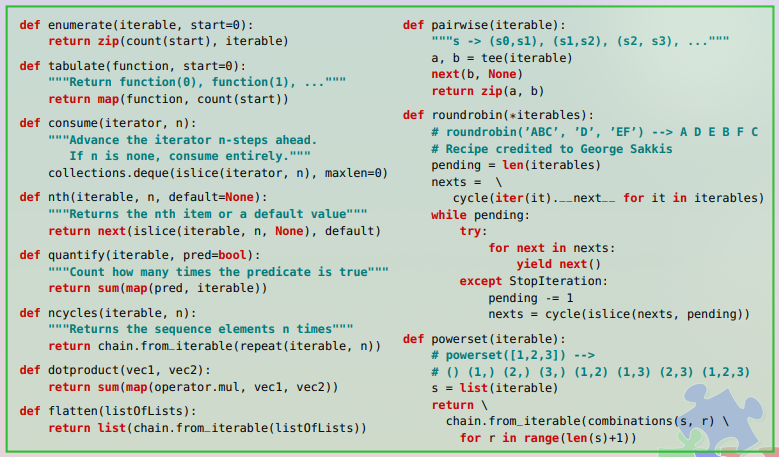
\includegraphics[scale=0.7]{5-iterators-the-module-itertools}
\end{center}

\subsubsection{The module itertools: precooked recipes}

\begin{center}
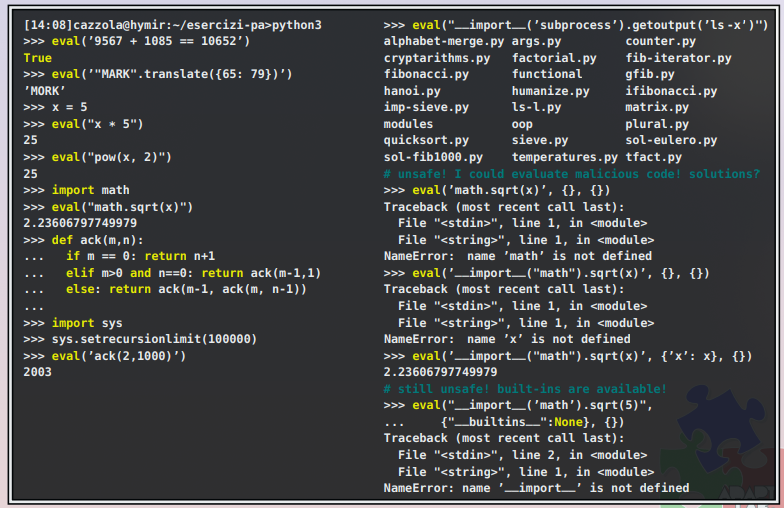
\includegraphics[scale=0.7]{6-iterators-eval}
\end{center}


